\singlespacing
\mychapter{0}{Apéndice II: Platina \href{https://github.com/jrr1984/open\_frame\_XYStage/tree/master/3dprintedparts/STLs}{\faCubes}.}
\label{chap:platine}
\spacing{1.5}

\pagestyle{plain}

\hspace{0.5cm}En este apéndice se describe el desarrollo y la implementación de la platina en el equipo. Una imagen representativa de una de las primeras versiones de la platina con dos grados de libertad se muestra en la Figura \ref{fig:plato0}.


\begin{figure}[H]
	\centering
	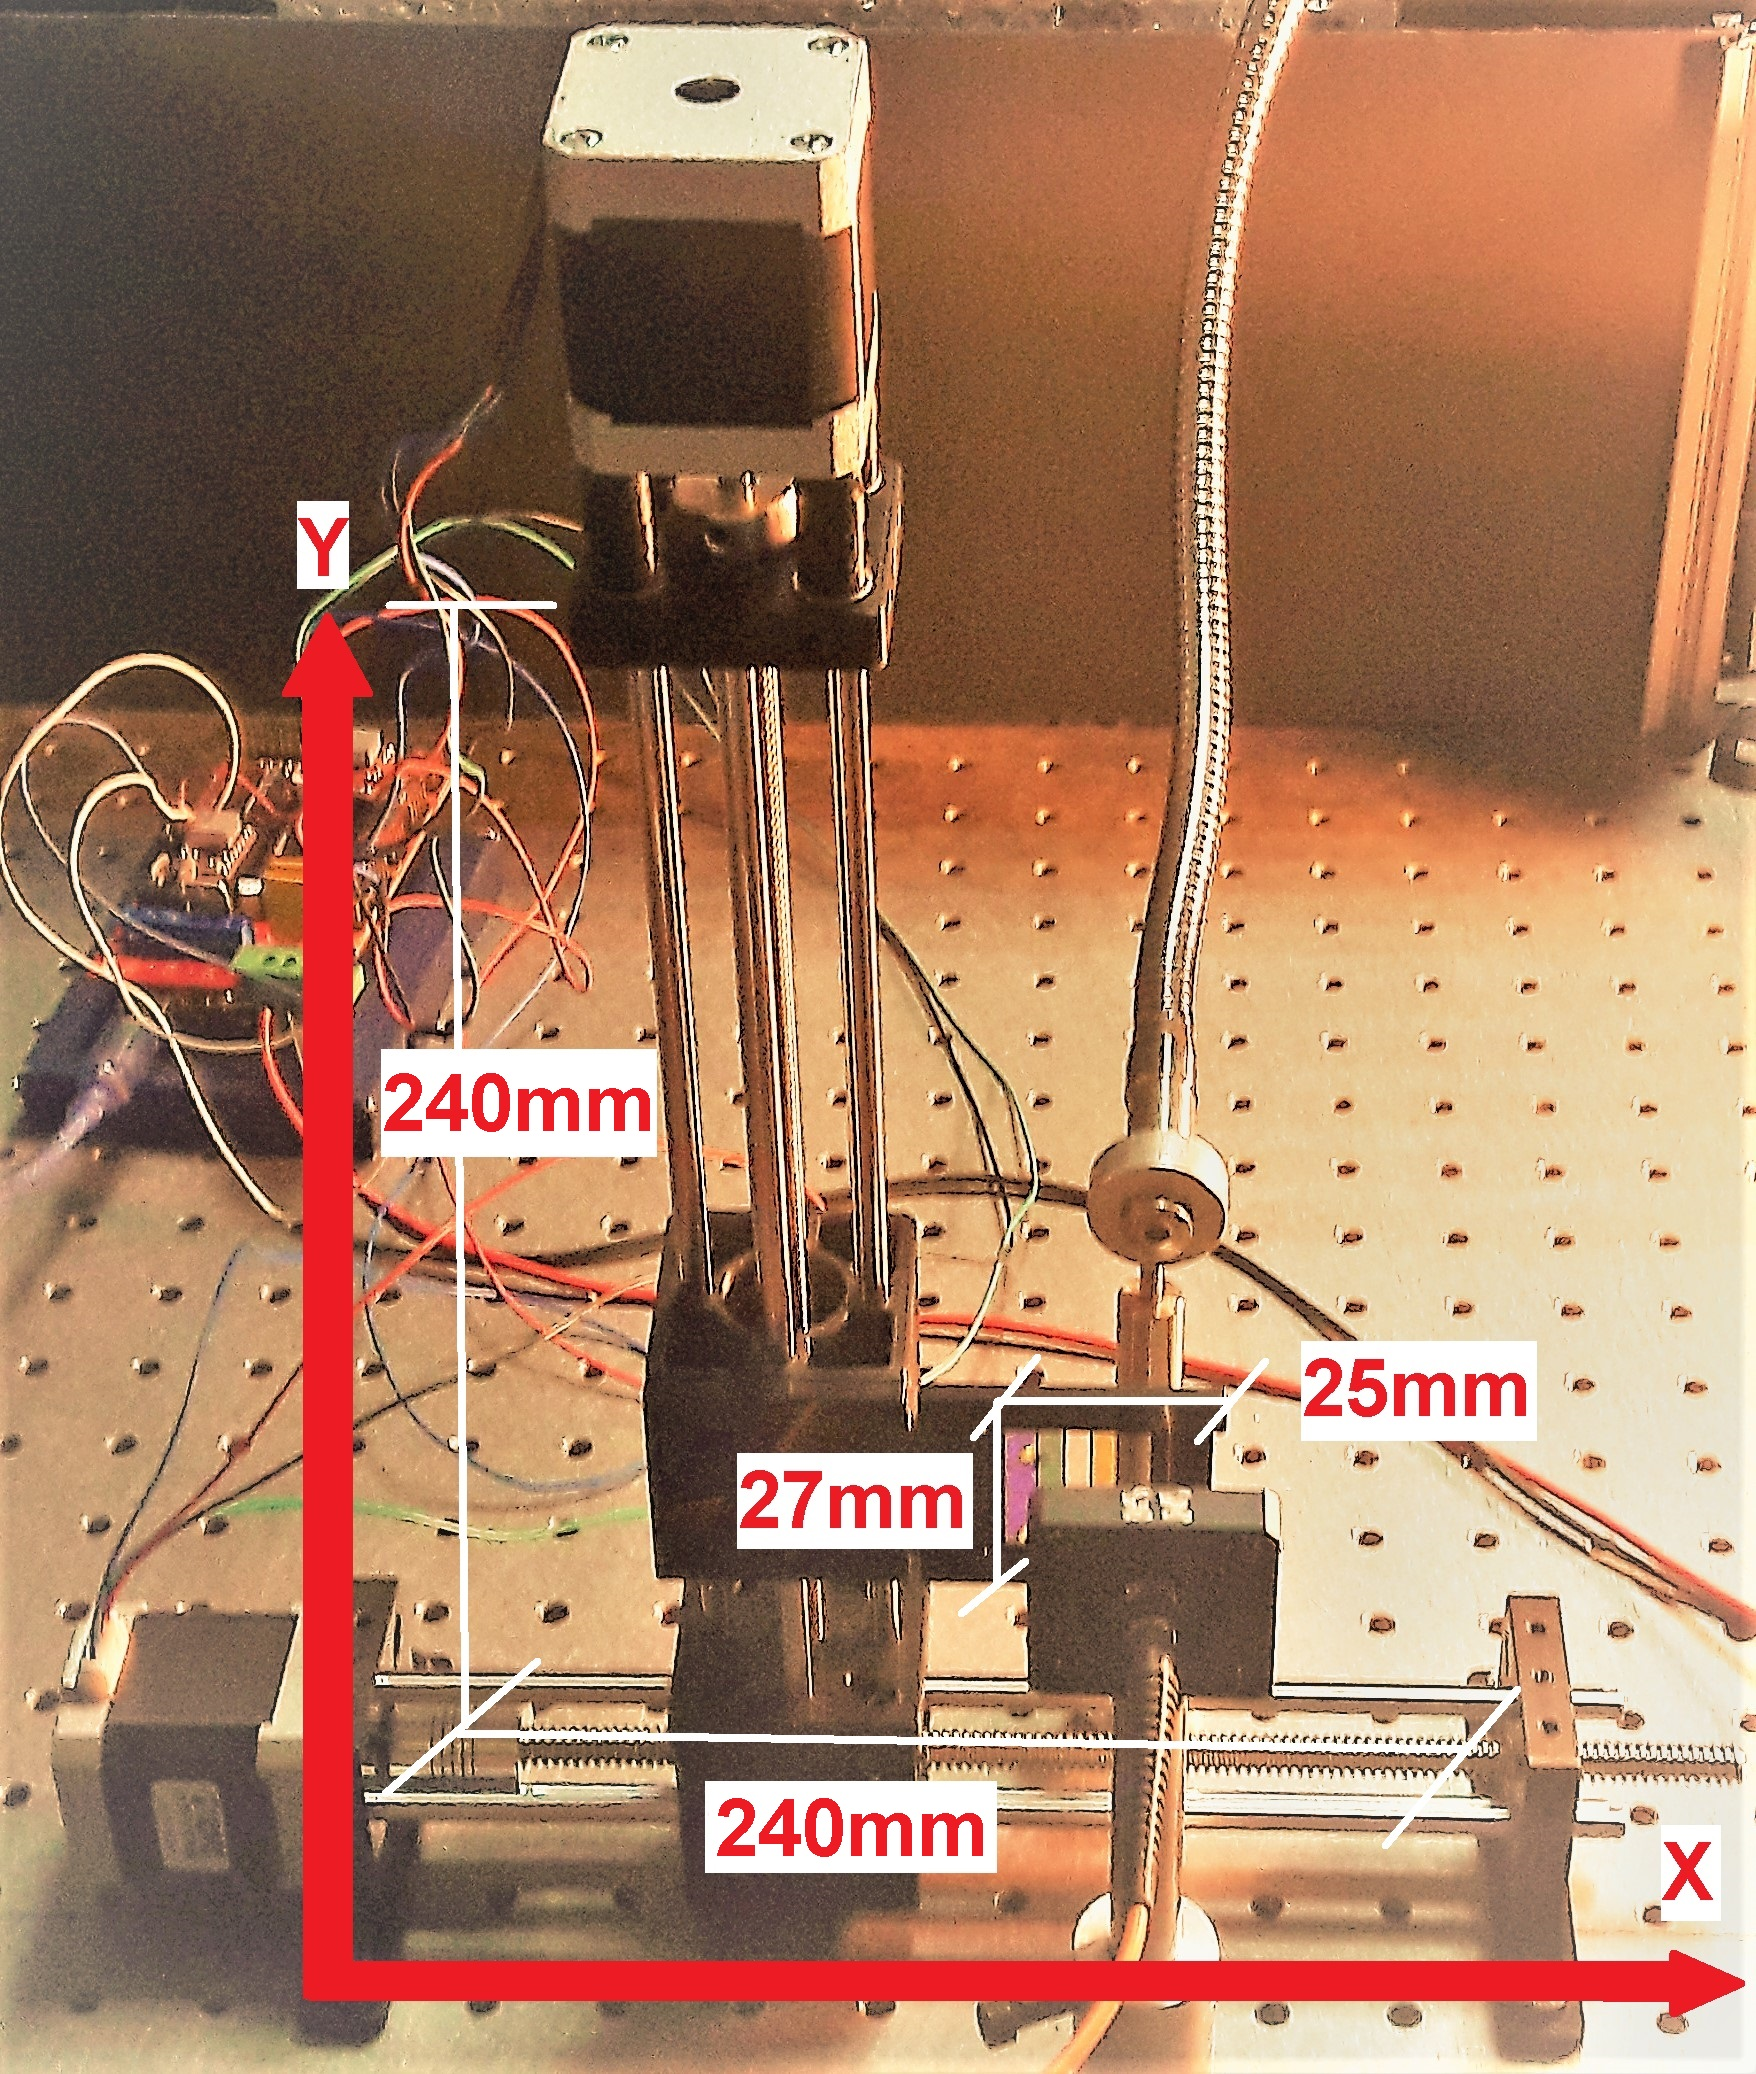
\includegraphics[scale=0.15]{Figs/microespectrometro/stageearly.jpg}
	\caption{Imagen de una de las primeras versiones de la platina motorizada con dos grados de libertad.}
	\label{fig:plato0}
\end{figure}


La construcción y desarrollo de la platina motorizada del microespectrómetro consistió de las siguientes etapas de prototipado:

\begin{enumerate}
\item Investigación previa de la literatura sobre platinas de microscopía de bajo costo y factibles para integrar al prototipo.
\item Elección de los componentes y materiales en función de la oferta local en Argentina.
\item De acuerdo al ítem 2, se realizó un dimensionamiento de la platina y se determinó el recorrido total de cada uno de los grados de libertad. Esto permitió evaluar la factibilidad y aplicabilidad de la plataforma a desarrollar.
\item En conjunto con el diseñador industrial Federico Armesto se diseñaron las piezas de impresión 3D y se montó el primer eje de la platina. Se desarrolló la electrónica y el \textit{software} necesarios.
\item Una vez optimizado el diseño del primer eje, se montó el segundo eje de la platina. Se extendió el software y se integraron finales de carrera.
\item Desarrollo del \textit{software} de control de la platina. Calibración preliminar.
\end{enumerate}

A continuación se describen algunas consideraciones técnicas y de diseño que se tuvieron en cuenta para el desarrollo de la platina motorizada y que podrían ser de utilidad para otros laboratorios que quisieran replicar la plataforma que aquí se presenta, realizar una adaptación ó simplemente como fuente de consulta.

Respecto de la revisión de la literatura sobre platinas de microscopía de bajo costo y factibles para el prototipo, se consultaron  los prototipos cuyos proyectos hayan sido desarrollados bajo la modalidad \textit{open source} tanto para la distribución del diseño de las piezas 3D como del \textit{software}, dentro de las cuales se destacan \cite{schaa}(\textit{LabView}, EUR 250) y \cite{campbells}(Instrucciones vía puerto serie en \textit{Matlab}, \textit{LabView} y \textit{python}, USD 1000). Dichas propuestas son también denominadas en cierto contexto DIY (\textit{Do it yourself}) ya que contienen toda la documentación y herramientas necesarias para que cualquier usuario con presupuesto y acceso a los mismos componentes pueda reproducir el proyecto. Además de estos proyectos se consultaron múltiples platinas de microscopía comerciales, donde en sus páginas la mayoría de los fabricantes distribuyen los planos de diseño, las piezas 3D libres para modificar, etc (\href{https://www.thorlabs.com/newgrouppage9.cfm?objectgroup\_id=2132}{NRT150 Thorlabs} USD 2456 x 2, \href{https://www.edmundoptics.com/p/150mm-motorized-stage/16419/}{\#59-747 EO} USD 2095 x 2). Ahora bien, hasta la fecha de escritura de este trabajo no se registraban prototipos de platinas motorizadas de microscopía desarrolladas en laboratorios del país como la que aquí se presenta por lo cual por medio de la presente se comparten las piezas de diseño 3D y el \textit{software} necesarios para poder replicarla y extender sus prestaciones. El costo total aproximado de la platina aquí desarrollada fue de USD 200.

El tipo de platina motorizada a desarrollar dependió del presupuesto, de la oferta local de los componentes y de los requerimientos mecánicos de precisión, longitud de recorrido y repetibilidad. Estos tres conceptos se encontraban relacionados fuertemente entre sí. Si bien se podrian haber comprado los componentes de la platina en el exterior del país, la futura necesidad de comprar nuevamente alguno de los componentes debido al desgaste ó rotura de los mismos, hacen de esta implementación de la compra una mala práctica del prototipado. En este sentido se eligieron componentes masivos en el país, los cuales se podían conseguir fácilmente sus repuestos en caso de necesidad. Al mismo tiempo, los componentes masivos son los que tienen un menor costo debido a su mayor demanda.

Se consultaron fundamentalmente tres proveedores de componentes mecánicos y de electrónica, de la ciudad de Buenos Aires y de la provincia de Buenos Aires: \href{https://3dinsumos.com.ar/}{3DInsumos} (Caseros, Buenos Aires), \href{https://ingia.com.ar/}{Ingia Automatización} (Saavedra, C.A.B.A.) y \href{https://candy-ho.com/}{Candy-Ho} (Villa Martelli, C.A.B.A.). A partir de la oferta de estos y otros proveedores se eligieron los componentes de la platina tomando como idea de diseño e implementación la platina de \cite{schaa} que por su bajo costo y la utilización de piezas 3D que facilitaban el prototipado rápido (dependiendo de la disponibilidad de una impresora 3D), hacían de esa propuesta la más indicada para ser implementada.

Los componentes principales de la platina son el motor paso a paso y el sistema de transmisión que transforma la rotación del motor en un desplazamiento lineal. Uno de los motores paso a paso más populares del mercado sino el más popular es el \href{https://www.pololu.com/product/1200}{NEMA 17} que es ampliamente utilizado en impresoras 3D y CNC. Por este motivo se eligió ese motor en lugar del \href{https://www.pololu.com/product/1204}{NEMA 8} utilizado en \cite{schaa}, que sólo se podía conseguir haciendo un pedido al exterior lo que encarece su costo y alarga notablemente los tiempos de prototipado.

De la familia de motores paso a paso NEMA 17 (Ver Figura \ref{fig:acm} \textbf{A}) existen distintos modelos dependiendo los requerimientos de torque y de resolución fundamentalmente. El torque no fue una limitante para la elección del modelo con lo cual en función de las distintas opciones de torque se priorizó el de menor precio. Ahora bien, respecto de la precisión existen dos modelos con pasos mínimos de rotación de 1.8 grados y de 0.9 grados, con lo cual se tienen 200 y 400 pasos por revolución respectivamente. Se evaluó la oferta disponible en el mercado y se eligieron motores NEMA 17 con un paso mínimo de 0.9 grados con el fin de obtener la mayor resolución en el desplazamiento lineal, a pesar de que su costo era mayor.

A la elección del motor, le sigue la elección del sistema de transmisión donde existen múltiples opciones dependiendo de la precisión, entre ellas las correa dentadas con poleas, las varillas roscadas, los husillos de bolas, etc. De acuerdo a \cite{schaa} se optó por una varilla roscada masiva en el mercado del tipo \href{https://www.mcmaster.com/acme-screws/acme-lead-screws-and-nuts/}{ACME} (Ver Figura \ref{fig:acm} \textbf{B}) de un diámetro de 8 mm y con un paso (\textit{pitch}) de 2 mm, es decir que por cada revolución completa del motor se realiza un desplazamiento lineal de 2 mm. La rotación del motor paso a paso es transferida a la varilla roscada ACME por medio de un acople sólido con agujeros para prisioneros M3 equidistanciados a 180° para que la varilla roscada quede centrada, que fue diseñado (Ver \href{https://github.com/jrr1984/open\_frame\_XYStage/blob/master/3dprintedparts/STLs/acopleRIGIDO.STL}{\faCubes$_{1}$}).
\begin{figure}[H]
\centering
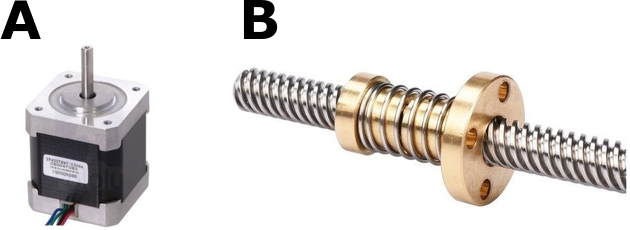
\includegraphics[scale=0.35]{Figs/microespectrometro/nemoacme.png}
\caption{\textbf{A}: Motor paso a paso \href{https://www.pololu.com/product/1200}{NEMA 17} con una resolución de 400 pasos por revolución (0.9° por paso). \textbf{B}: Varilla roscada del tipo \href{https://www.mcmaster.com/acme-screws/acme-lead-screws-and-nuts/}{ACME} con un paso (\textit{pitch}) de 2 mm  y un diámetro de 8 mm, junto con una tuerca \textit{anti-backslash}.}
\label{fig:acm}
\end{figure}

Además del sistema de transmisión se tuvo que elegir un sistema de desplazamiento que es el que permite el movimiento de los ejes de la platina. Se eligió la opción más utilizada en impresoras 3D en el que se utilizan sistemas lineales con barras rectificadas de acero de 6mm de diámetro y rodamientos lineales \href{https://uk.misumi-ec.com/vona2/detail/221000091678/?HissuCode=LM6LUU}{LM6LUU}. Dichos rodamientos y la tuerca \textit{antibackslash} fueron montados sobre un cubo diseñado e impreso con una impresora 3D (Ver \href{https://github.com/jrr1984/open_frame_XYStage/blob/master/3dprintedparts/STLs/cuboconLM6UU_2demarzo.STL}{\faCubes$_{2}$}) que realizó los desplazamientos lineales al deslizarse sobre las barras de acero.

La resolución espacial mecánica es el mínimo desplazamiento de cada uno de los ejes de la platina. La misma viene dada teóricamente por la siguiente ecuación:
\begin{equation}
\text{Resolución} [\mu m / paso] = \frac{\text{\textit{Pitch} del ACME}}{\text{\# de pasos por revolución del motor}} = \frac{2 mm}{400 pasos} = \frac{5 \mu m}{paso}
\end{equation}

Además esta resolución fue modificada por medio de la electrónica que controla los motores paso a paso implementando una técnica que se conoce como \textit{microstepping} \cite{7806244}. Esta técnica permite al motor realizar rotaciones de ángulos menores al paso mínimo del motor, con lo cual se mejora la resolución ya que se puede subdividir un paso completo del motor en 2,4,8,16 e incluso hasta en 32 pasos (teóricos). Al mismo tiempo se reduce el ruido del motor y el movimiento del mismo se suaviza. La técnica es impelementada por el controlador de corriente que utiliza un algoritmo que a su salida envía una modulación sinusoidal discretizada de la corriente, donde cada paso de dicha modulación sinusoidal consiste de un micropaso y el período de la señal es igual al paso completo original del motor.

Los dos controladores de corriente de los motores paso a paso más populares con la capacidad de aplicar \textit{microstepping} son el \href{https://www.pololu.com/product/2133}{DRV8825}(hasta 32 micropasos y 2.5 A) y el \href{https://www.pololu.com/product/1182}{A4988} (hasta 16 micropasos y 2 A). Se eligió finalmente para la platina el \textit{driver} A4988 (Ver Figura \ref{fig:elec} \textbf{A}) y se limitó la máxima corriente que podía entregar de acuerdo al consumo observado de los motores en condiciones de operación normales, ajustando el potenciómetro (Ver Figura \ref{fig:elec} \textbf{A}) a partir de la medición de una tensión de referencia de acuerdo a las especificaciones del manual del fabricante \cite{a4988}.

Se utilizó un \href{https://store.arduino.cc/usa/mega-2560-r3}{\textit{Arduino MEGA 2560}} para controlar la lógica de la platina vía el puerto USB de una computadora y se le montó a los pines hembra del arduino un \textit{shield} \href{https://reprap.org/wiki/RAMPS_1.4}{\textit{RAMPS 1.4}} donde se colocaron los \textit{drivers} de los motores, las conexiones de los finales de carrera y el \textit{joystick} (Ver Figura \ref{fig:elec} \textbf{B}). La RAMPS fue alimentada de forma independiente con una fuente de tensión.

\begin{figure}[H]
\centering
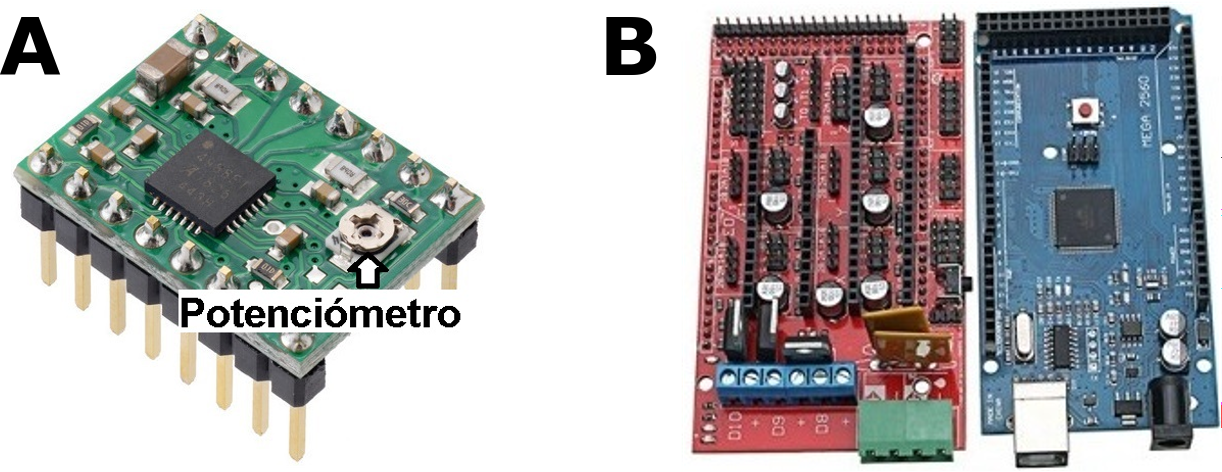
\includegraphics[scale=0.18]{Figs/microespectrometro/rampa4.png}
\caption{\textbf{A} Controlador de los motores paso a paso A4988. \textbf{B} \href{https://store.arduino.cc/usa/mega-2560-r3}{\textit{Arduino MEGA 2560}} a la derecha en azul y \href{https://reprap.org/wiki/RAMPS_1.4}{\textit{Shield RAMPS 1.4}} a la izquierda en rojo.}
\label{fig:elec}
\end{figure}



Antes de realizar la compra de los componentes necesarios para montar el primer eje se determinó el recorrido total de cada uno de los grados de libertad de la platina de acuerdo a la oferta de los proveedores. Por ejemplo, existen comercialmente distintas longitudes de varillas roscadas ACME y se eligió una longitud de la misma de 500 mm, de forma tal que al cortar dicha varilla se pueda obtener las dos varillas necesarias para cada eje de la platina, cada una de 250 mm de largo. El mismo razonamiento fue aplicado a las varillas de acero de 6 mm de diámetro, para las cuales se compraron dos varillas de 1 metro que cada una fue cortada en cuatro partes de 250 mm cada una. De esta manera, se realizó un diagrama con las dimensiones y la longitud de recorrido estimada de uno de los ejes de la platina con el software \textit{Solidworks} como se muestra en la Figura \ref{fig:dimejee}.

\begin{figure}[H]
	\centering
	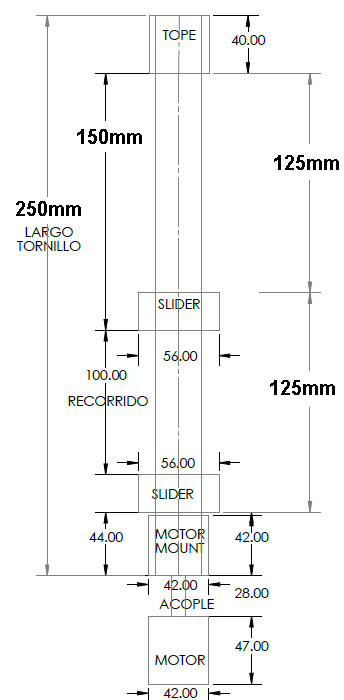
\includegraphics[scale=0.6]{Figs/microespectrometro/dimensio.png}
	\caption{Estimación del recorrido de uno de los ejes de la platina.}
	\label{fig:dimejee}
\end{figure}

El objetivo de esta etapa del prototipado fue el de evaluar la factibilidad y aplicabilidad de la platina para poder desplazar al filtro respecto de la fuente de luz y del espectrómetro de manera tal de poder obtener una medición del espectro en cualquier región del filtro deseada. Luego de realizar el dimensionamiento, se decidió montar el eje $\textit{x}$ de la platina únicamente. En la Figura \ref{fig:dis} \textbf{A} se muestra el diseño del eje $\textit{x}$ realizado con el software libre \textit{Fusion 360} y en la Figura \ref{fig:dis} \textbf{B} se muestra un montaje preliminar de dicho eje\footnote{Se imprimió inicialmente una porción del cubo diseñado como prueba preliminar, ya que la impresión del cubo completa podía tomar más de 10 horas. Resultó importante realizar pruebas por etapas para reducir los tiempos de prototipado.}. 

\begin{figure}[H]
\centering
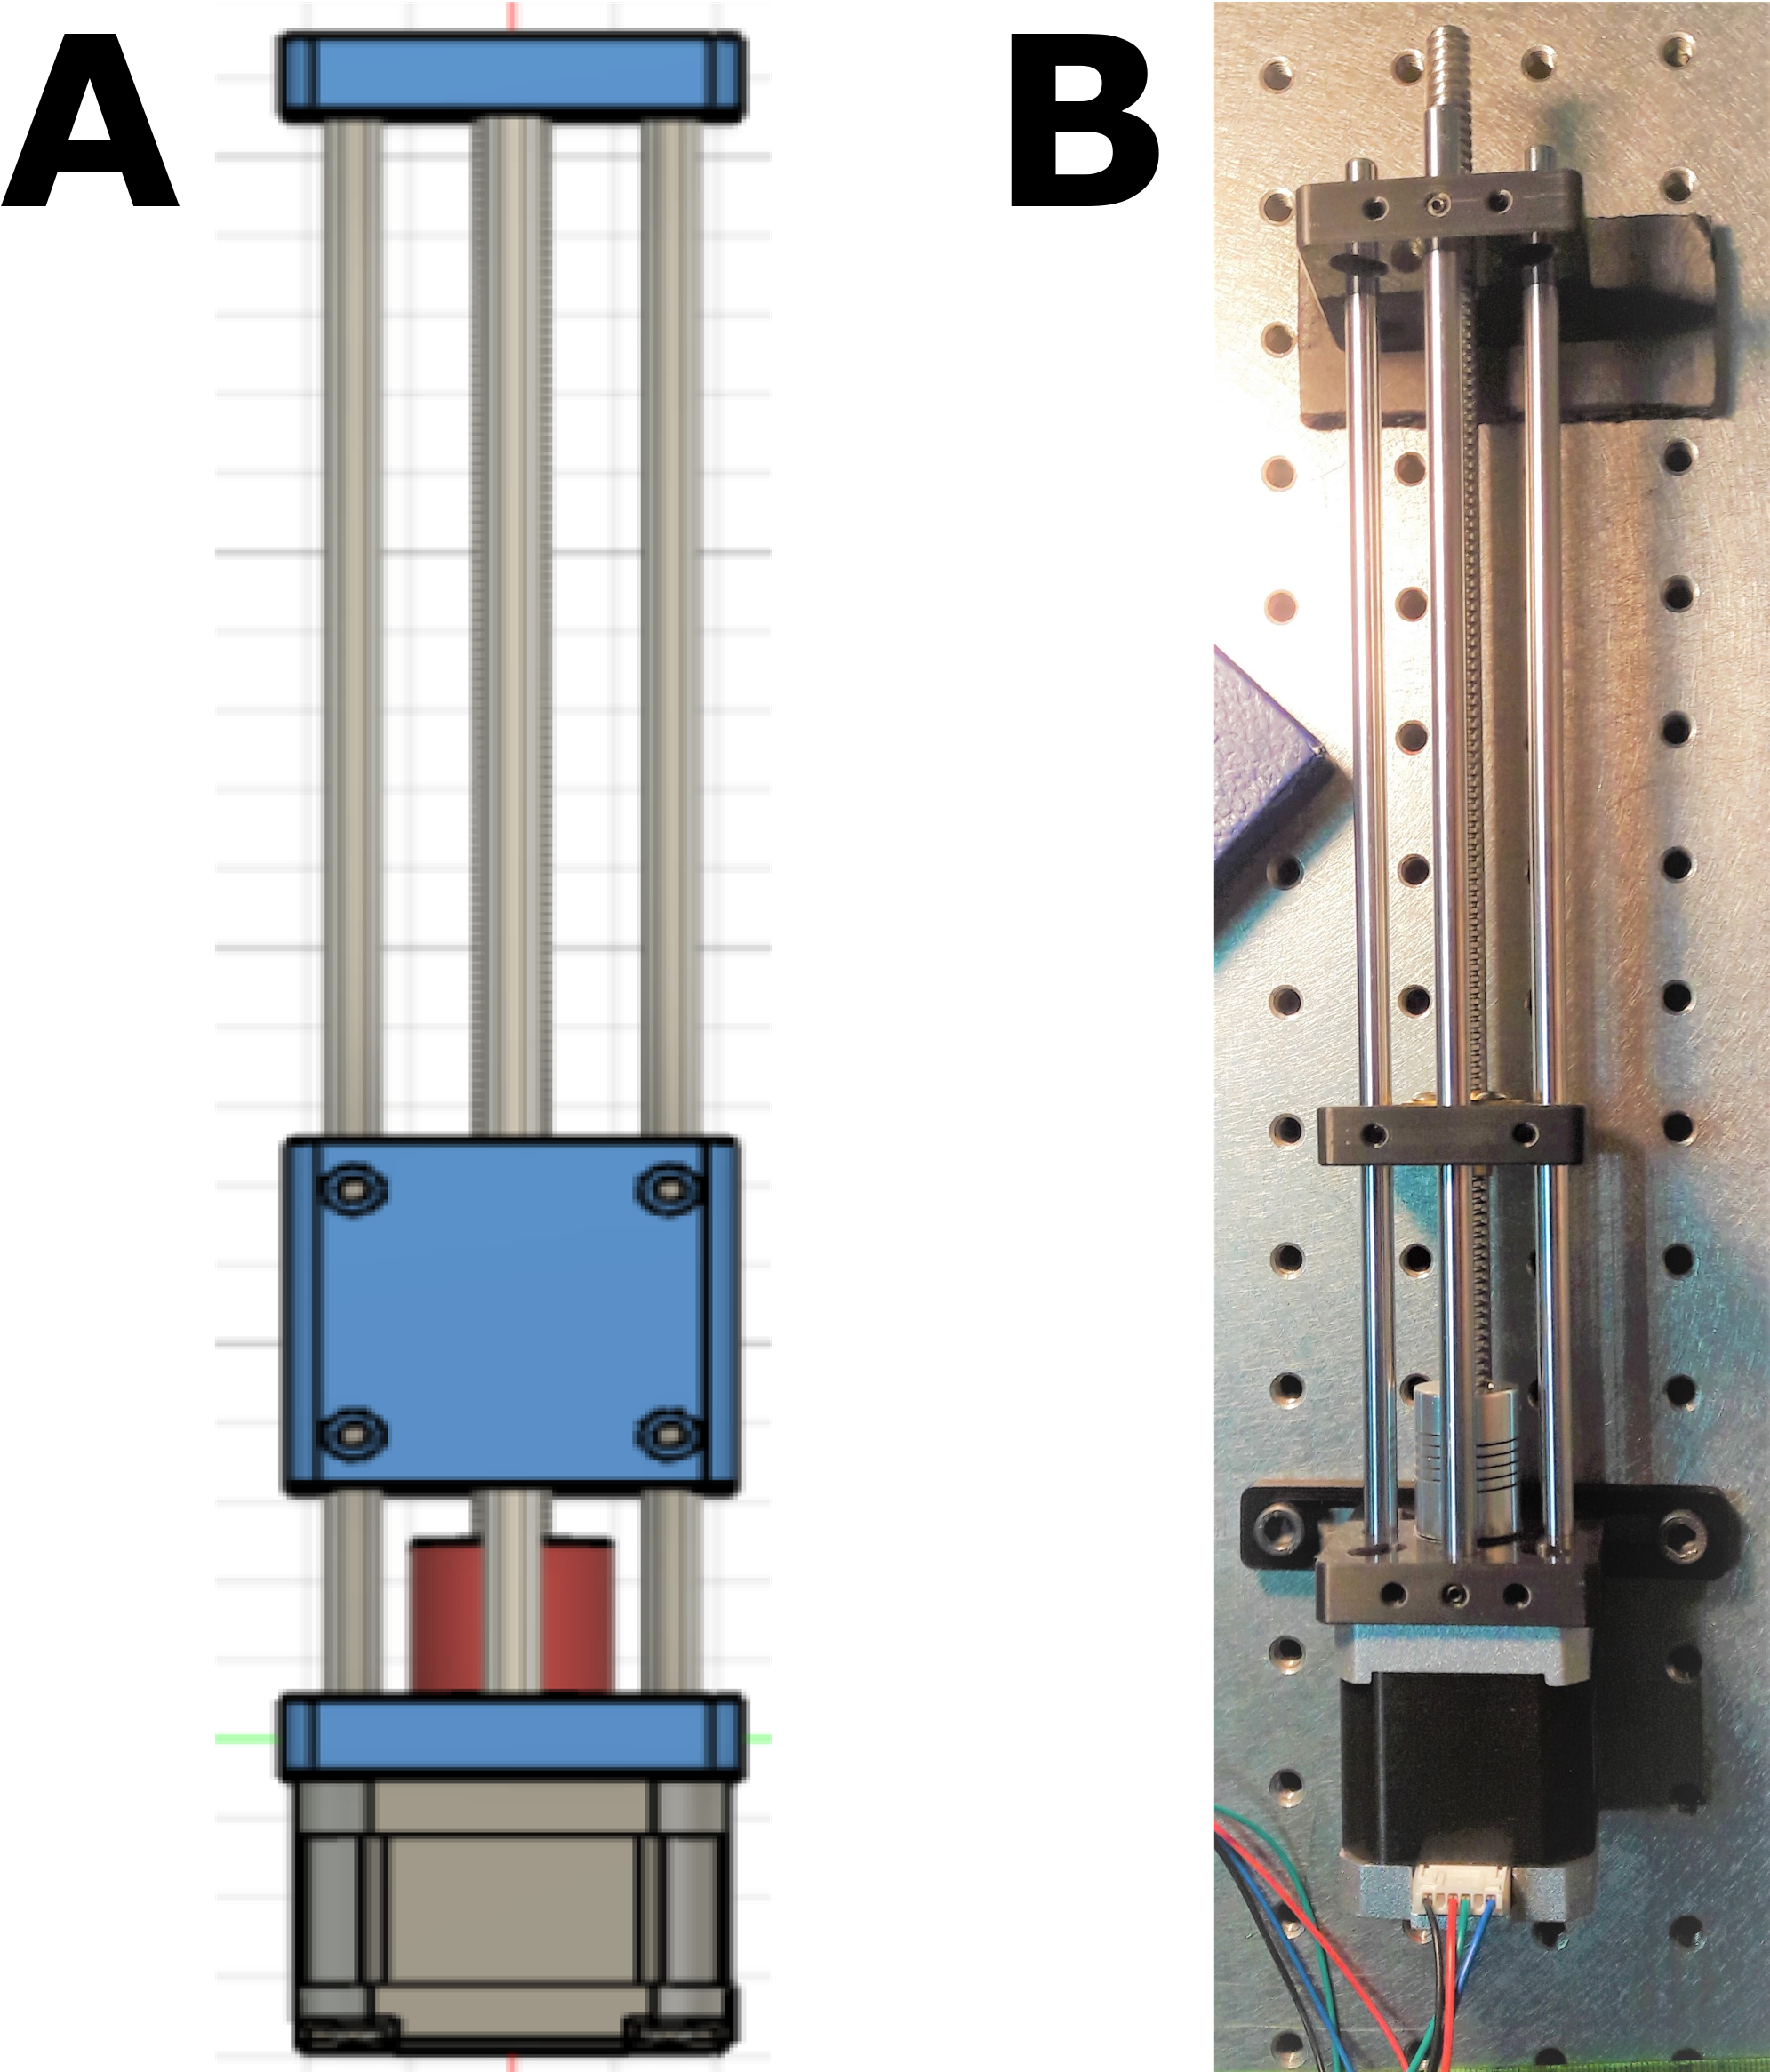
\includegraphics[scale=0.1]{Figs/microespectrometro/111eje.png}
\caption{\textbf{A}: Diseño de las piezas 3D del eje $\textit{x}$ de la platina [\href{https://github.com/jrr1984/open_frame_XYStage/blob/master/3dprintedparts/STLs/Ejexpreliminar.stl}{\faCubes$_{3}$}]. \textbf{B}: Montaje preliminar del eje $\textit{x}$ de la platina.}
\label{fig:dis}
\end{figure}

Luego de optimizar el diseño y montaje del primer eje, se montó el eje $\textit{y}$ compuesto por las mismas piezas 3D que el eje $\textit{x}$, como se muestra en la Figura \ref{fig:eee}. En este sentido se hace notar que el diseño propuesto resultó una solución completamente modular y que la configuración de los ejes aquí adoptada puede ser modificada a otras de acuerdo a las necesidades del usuario final. 
 
\begin{figure}[H]
\centering
\includegraphics[width=1.0\textwidth]{Figs/microespectrometro/platinafinel.png}	
\caption{\textbf{A}: Diseño preliminar de los dos ejes de la platina. \textbf{B}: Montaje final de la de la platina.}
\label{fig:eee}
\end{figure}

%%%%%%%%%%%%%%%%%%%%%%%%%%%%%%%%%%%%%%%%%%%%%%%%%%%%%%%%%%%%%%%%%%%%%%%%%%%%%%%%%%%%%%%%%%%%%%%%%%%%%%%%%%%%%%
%%%%%%%%%%%%%%%%%%%%%%%%%%%%%%%%%%%%%%%%%%%%%%%%%%%%%%%%%%%%%%%%%%%%%%%%%%%%%%%%%%%%%%%%%%%%%%%%%%%%%%%%%%%%%%

\singlespacing
\section*{\textit{Software} de control de la platina \href{https://github.com/jrr1984/open\_frame\_XYStage}{\faGithub$_{\text{A.II}}$}  y calibración preliminar}
\label{sec:softcalib}
\spacing{1.5}

\hspace{0.5cm}Se desarrolló un \textit{software} de control de la platina que fue integrado al \textit{software} de control del espectrómetro y de la cámara. En [\cite{campbells},\href{https://github.com/raacampbell/openstage/tree/master/serialInterfaceScripts}{\faGithub$_{\text{A.II}.2}$}] se desarrollaron instrucciones específicas de comandos a ejecutar vía el puerto serie al que se conectó el arduino que controla la lógica de la platina, por medio de los lenguajes de programación \textit{Matlab}, \textit{LabView} y \textit{python}. En el proyecto \textit{open source} \href{https://www.youtube.com/watch?v=Lm8oprDhAnQ}{RDL} [\href{https://forum.arduino.cc/index.php?topic=469343}{\faCode}] se desarrolló un \textit{software} de comandos muy exhaustivo a ejecutar únicamente por el puerto serie de arduino.

El \textit{software} de control de la platina fue organizado como se muestra en la Figura \ref{fig:cnpl}. A nivel del microcontrolador las instrucciones a los \textit{drivers} que regulan la corriente de los motores y le envían los pulsos PWM para que realicen la cantidad de pasos elegidos fueron desarrolladas con la librería de \textit{Arduino} \href{https://www.airspayce.com/mikem/arduino/AccelStepper/}{AccelStepper}. Dichas instrucciones escritas en el lenguaje de programación propio de arduino incluyen métodos para asignarle las posiciones de los motores, para leer las posiciones de los motores, para prenderlos, apagarlos, determinar si llegaron a la posición asignada ó no, para ponerlos en la posición inicial de la platina, para leer los finales de carrera, etc. Todos los métodos escritos se pueden ver en el \textit{header} del \textit{driver} desarrollado [\href{https://github.com/jrr1984/open_frame_XYStage/tree/master/ino_main}{\faGithub$_{\text{A.II}.3}$}].
Ahora bien, para poder integrar el control de la platina con el espectrómetro y con la cámara se tuvo que establecer una comunicación por medio de mensajes a través del puerto serie de la computadora. Para ello se utilizó la librería \href{https://github.com/kroimon/Arduino-SerialCommand}{\textit{SerialCommand}} que permitió unir la lógica a nivel del microcontrolador del \textit{Arduino} con la lógica a nivel del procesador de la computadora. De esta manera, en el lenguaje de programación \textit{python} se escribió una clase [\href{https://github.com/jrr1984/open\_frame\_XYStage/blob/master/XYStage.py}{\faGithub$_{\text{A.II}.4}$}] con los mismos métodos de control de la platina escritos con la librería \textit{AccelStepper} en \textit{Arduino} de forma tal de enviar mensajes al puerto serie de la computadora que el \textit{Arduino} se encontraba constantemente escuchando. Así por ejemplo, desde \textit{python} se envía un mensaje al puerto serie para mover el motor del eje $\textit{x}$ una distancia de 2 mm, el \textit{Arduino} escucha ese mensaje y le envía los pulsos PWM al motor para realizar el desplazamiento. En la Sección \ref{sec:softadq} se explica el \textit{software} desarrollado para automatizar las mediciones que integró el control de la platina con el espectrómetro y la cámara.

\begin{figure}[H]
	\centering
	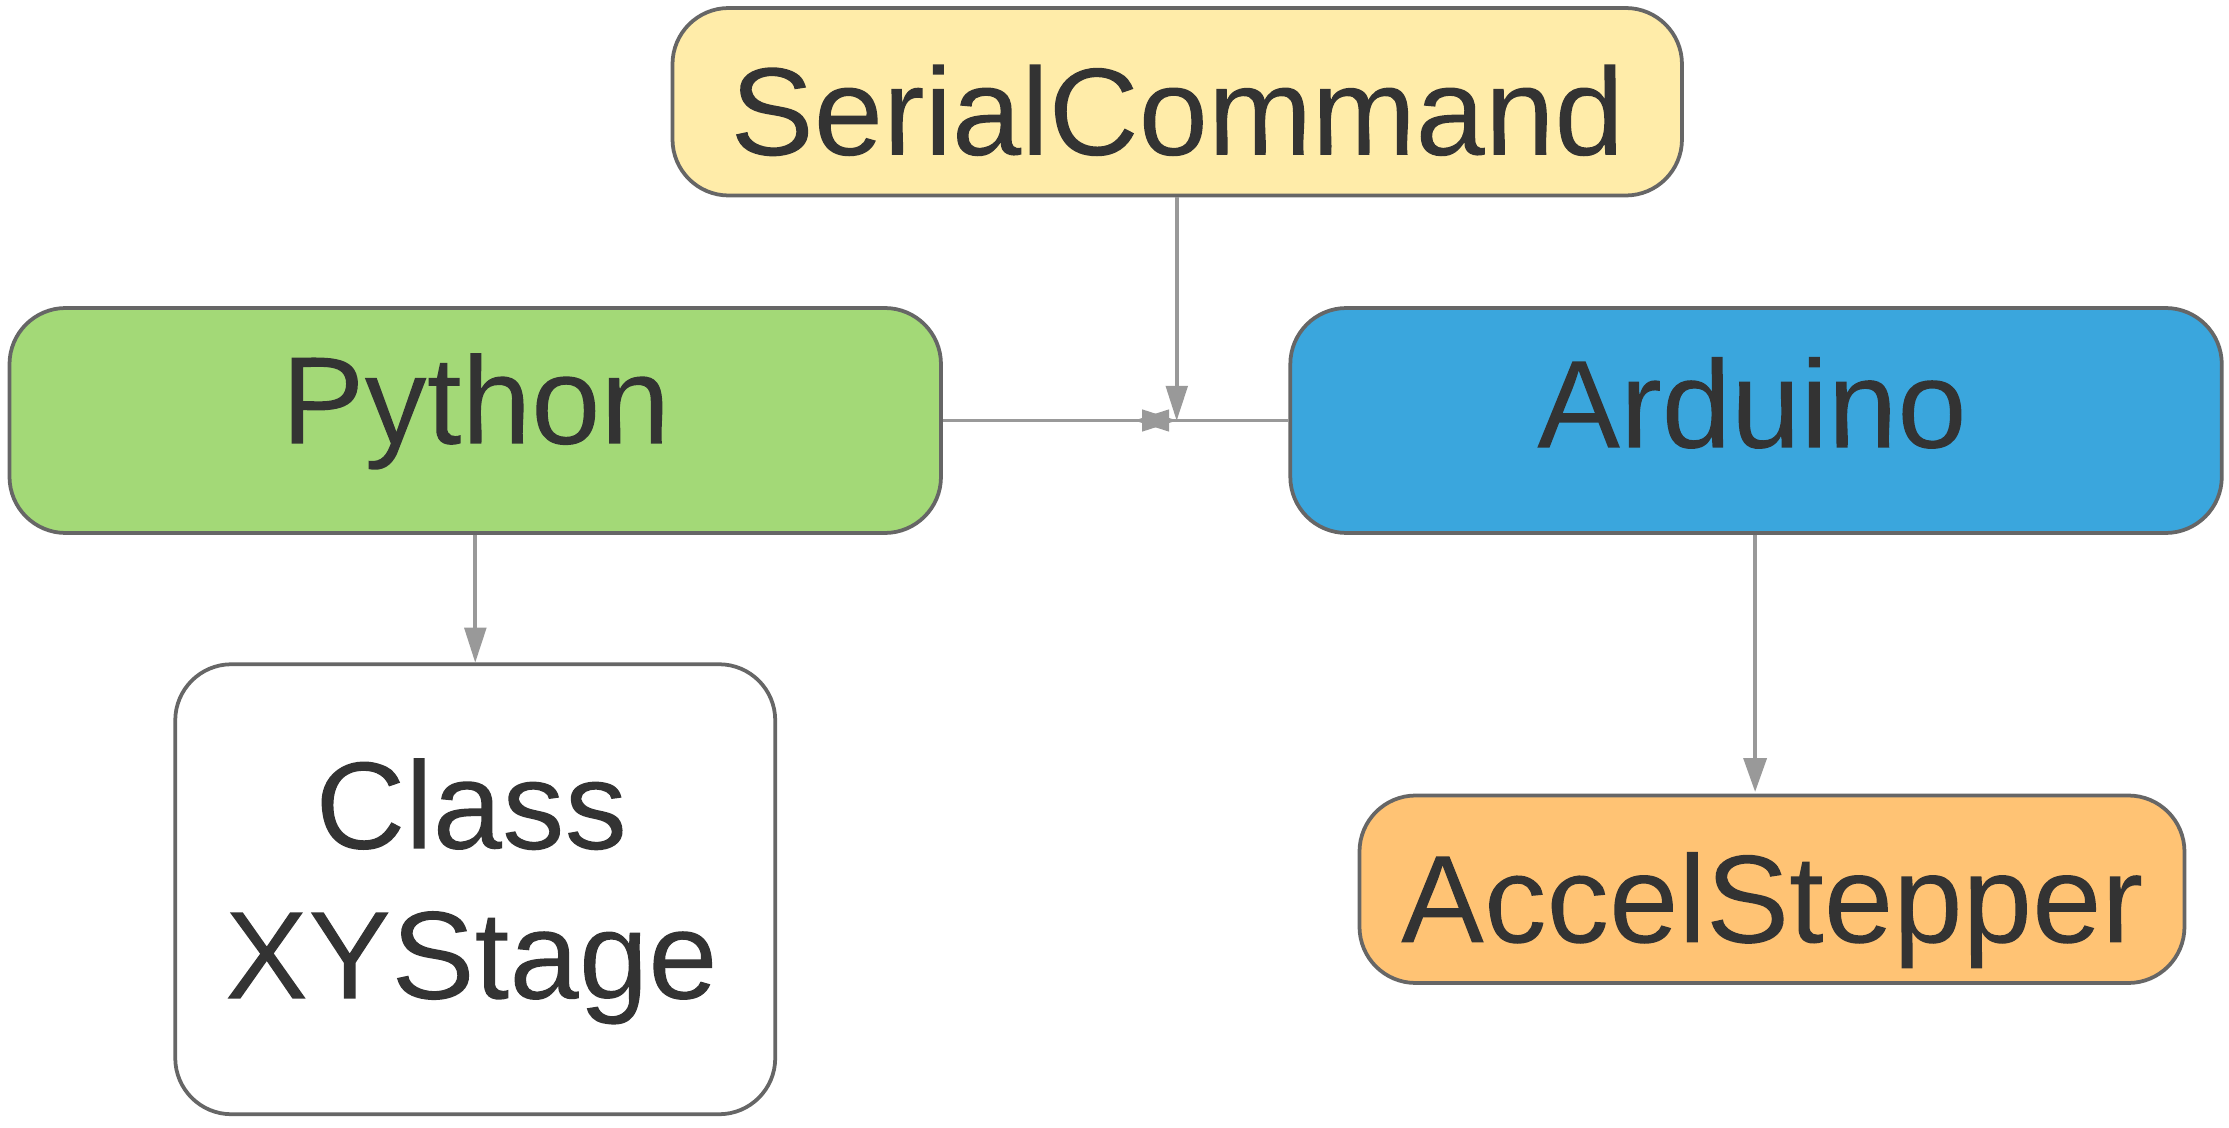
\includegraphics[scale=0.5]{Figs/microespectrometro/diagflujoplatina.png}
	\caption{Diagrama de la comunicación vía el puerto serie de la computadora entre el microcontrolador \textit{Arduino} y el proceso principal de la computadora programado en \textit{python} en el que se integró el espectrómetro y la cámara.}
	\label{fig:cnpl}
\end{figure}

Se realizó una calibración preliminar de la platina para determinar las incertezas de su resolución (mínimo paso de desplazamiento) que fueron luego utilizadas en la medición de la resolución espacial del microespectrómetro (Ver Sección \ref{sec:focoresol}). En el trabajo de \cite{schaa} realizaron una calibración de la platina adquiriendo sucesivas imágenes de una muestra calibrada de distancias (1951 USAF \textit{test target}), midiendo el desplazamiento relativo respecto de un punto de referencia situado en la imagen inicial adquirida. Al momento de escribir esta tesis se iba a realizar la calibración con el mismo método. El \textit{software} de adquisición ya se había desarrollado [\href{https://github.com/jrr1984/defectsGUI/blob/master/views.py}{\faGithub$_{\text{A.II}.4.2}$}] y ya se contaba con una pieza 3D impresa que hacía de soporte de una regla calibrada de microscopía colocada sobre un portamuestra, para realizar la calibración de la platina.

Ahora bien, en primer lugar se midió la precisión y exactitud de los desplazamientos de la platina en el orden de los milímetros. Para ello, por medio del \textit{software} desarrollado se asignaron posiciones a cada uno de los ejes de la platina y se comparó el valor medido con una regla metálica calibrada en milímetros con los valores asignados por \textit{software}. Se observó que la platina tenía exactitud en milímetros, ya que no se encontraron diferencias entre los valores de las posiciones asignadas y las posiciones medidas. Y, de la repetición de las mediciones se verificó su precisión en milímetros ya que las mediciones no presentaron dispersiones en los valores obtenidos.

Para medir la precisión y exactitud en el orden de los micrones, se utilizaron las mediciones del microespectrómetro como calibración preliminar. Se eligió la resolución teórica de 1 $\mu m$ del desplazamiento de cada eje de la platina en la adquisición de barridos de ciertas regiones del filtro con el microespectrómero. Dicha resolución representa el desplazamiento mínimo que cada eje de la platina podría realizar y su valor fue elegido considerando un compromiso entre el tiempo de duración de un barrido y la resolución del mismo ya que en cada paso de la platina se realiza una medición individual.
En primer lugar se utilizó como patrón de calibración la longitud del cromo que separa dos bandas del filtro medida con el microscopio Zeiss (Ver Sección \ref{subs:compl}). En la Figura \ref{fig:barrcromoo} se muestra el barrido del cromo entre las bandas roja y pancromática realizado con un paso de 1 $\mu m$.

\begin{figure}
	\centering
	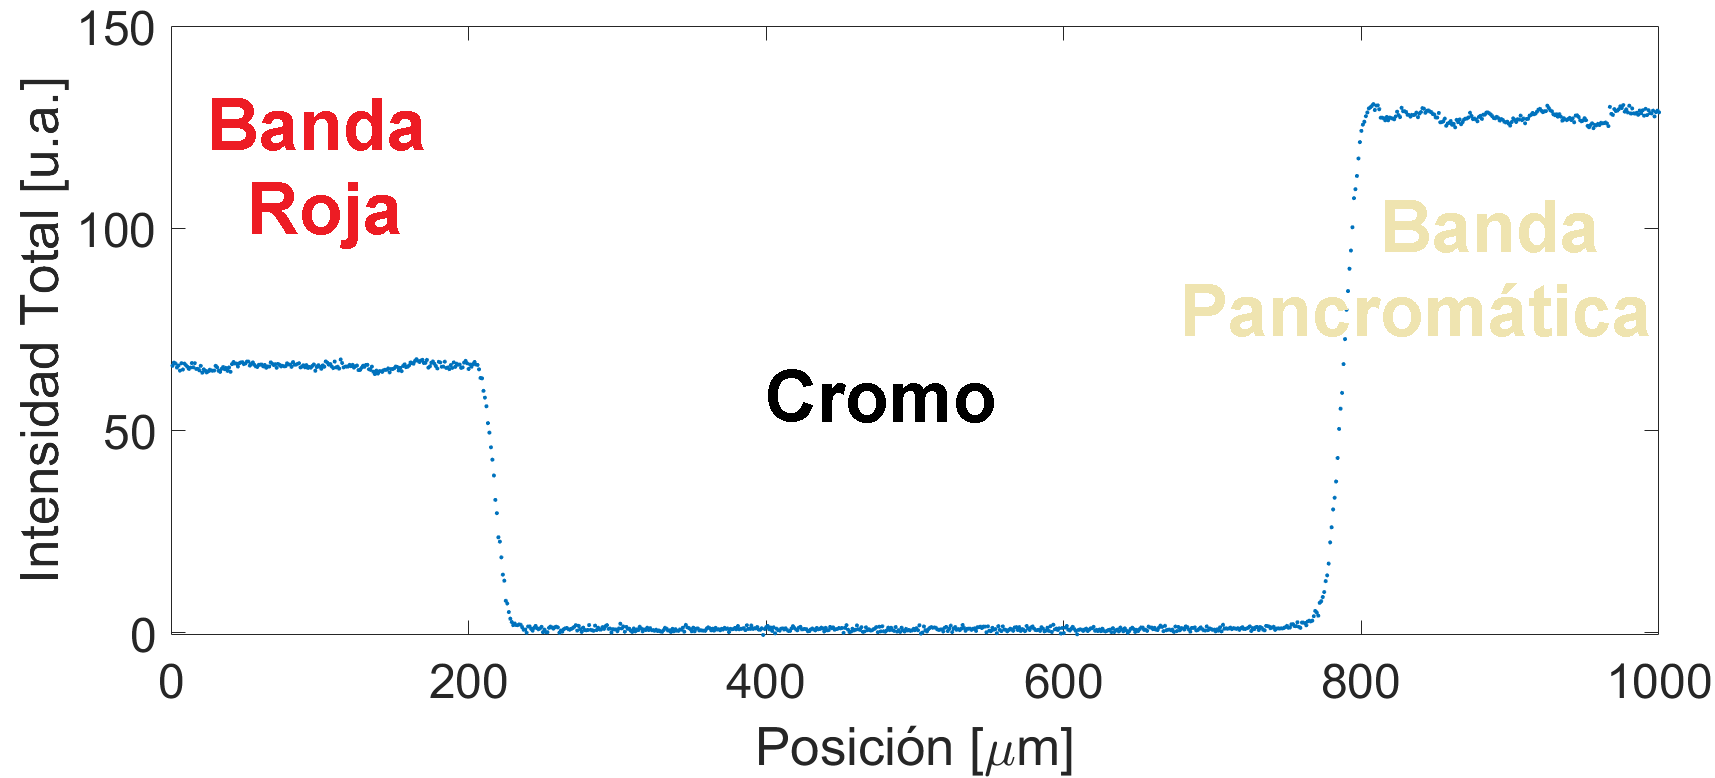
\includegraphics[width=1.0\columnwidth]{Figs/microespectrometro/barridocromocalib.png}
	\caption{Gráfico de la intensidad total detectada en función de la posición medida del filtro en un barrido lineal del cromo que separa las bandas roja de la pancromática.}
	\label{fig:barrcromoo}
\end{figure}

En el gráfico de la Figura \ref{fig:barrcromoo} se muestra la intensidad total detectada, esto es la suma de la intensidad detectada para cada longitud de onda del espectro medido, en función de la posición del filtro. El barrido fue lineal, es decir en una dimensión. Se asignó por \textit{software} a la platina un desplazamiento de 1000 $\mu m$, con un paso de 1 $\mu m$. En cada paso de la platina el microespectrómetro obtuvo una medición del espectro. Los espectros no fueron normalizados con la fuente de luz y es por eso que se puede observar un mayor valor de intensidad total para la banda pancromática que para la banda roja. El valor del cromo que separa la banda roja de la pancromática medido con el \textit{software} Fiji de una imagen completa del filtro adquirida con el microscopio Zeiss fue de $( 516 \pm 10)~ \mu m$.
Para determinar el valor medido de la longitud del cromo con el microespectrómetro se ajustó cada transición de una banda al cromo con la función error, \textit{erf(x)}, que es la integral del perfil gaussiano del haz de luz en una dimensión. La función utilizada para el ajuste fue, para la transición izquierda y derecha respectivamente:
\begin{equation}
\text{transición\_izquierda} (x,a,b,c) = \frac{a}{2}\hspace{2pt}.\hspace{2pt}erf\left(\sqrt{2}\hspace{1pt}.\hspace{1pt}\frac{(x-b)}{c}\right)
\label{eq:iz}
\end{equation}
\begin{equation}
\text{transición\_derecha} (x,a,b,c) = \frac{a}{2}\hspace{2pt}.\hspace{2pt}\left(1+erf\left(\sqrt{2}\hspace{1pt}.\hspace{1pt}\frac{(x-b)}{c}\right)\right),
\label{eq:der}
 \end{equation} para la transición izquierda [\ref{eq:iz}] y derecha [\ref{eq:der}] respectivamente. Así por ejemplo para el barrido de la Figura \ref{fig:barrcromoo} se ajustaron ambas transiciones como se muestra en las Figuras \ref{fig:ajustess} \textbf{A} y \textbf{B}. En azul se muestra el resultado del ajuste y los puntos rojos fueron datos eliminados de cada ajuste.
\begin{figure}[H]
\centering
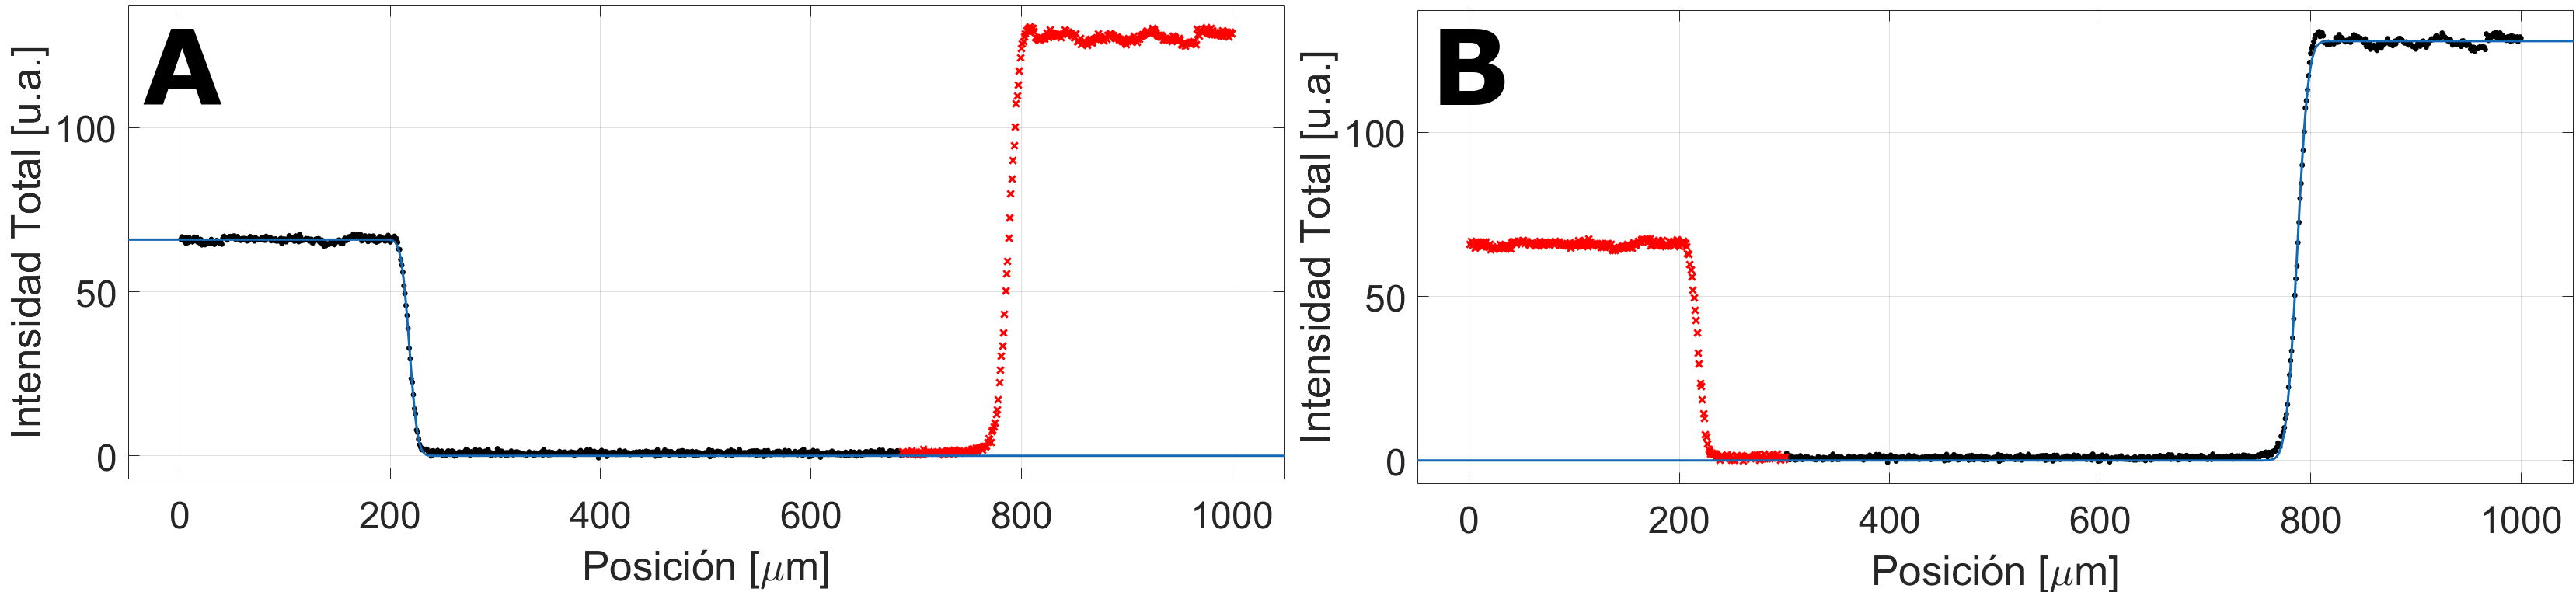
\includegraphics[width=1.0\textwidth]{Figs/microespectrometro/ajusteladosbarr.png}
\caption{\textbf{A} Ajuste de los datos de la transición de la banda roja al cromo por una función \textit{erf(x)}. \textbf{B} Ajuste de los datos de la transición del cromo a la banda pancromática por una función \textit{erf(x)}.}
\label{fig:ajustess}
\end{figure}

A partir de los parámetros del ajuste se determinó la longitud medida del cromo, $l_{cromo}$ de la siguiente manera:
\begin{equation}
l_{cromo} = (b_{der} - c_{der}) - (b_{izq} + c_{izq}),
\end{equation}
donde $b_{izq}, c_{izq}, b_{der} yc_{der}$ son los parámetros del ajuste de la transición entre la banda roja y el cromo (izq) y entre el cromo y la banda pancromática (der). Así, para el barrido que se muestra en la Figura \ref{fig:barrcromoo} se obtuvo una longitud del cromo igual a 540 micrones, con lo cual para esta medición la diferencia entre el valor medido con el microespectrómetro y el valor tomado como referencia medido con el Zeiss, fue del 5\%.

\newpage
\begin{figure}[H]
\begin{minipage}{0.47\textwidth}
\centering

\includegraphics[width=.7\textwidth,left]{Figs/microespectrometro/descarga.png}
\end{minipage}
\hfill
\begin{minipage}{0.47\textwidth}
\raggedleft
\Huge \textbf{XY(Z) Open Frame Stage}
\end{minipage}
\end{figure}

\texttt{Características principales y futuras mejoras:}

    \begin{itemize}
    \justifying
        \item Grados de libertad: 2. Ejes $\textit{x}$ e $\textit{y}$  .
        \item Longitud de recorrido de cada grado de libertad $>$ 240 mm.
        \item Motores paso a paso NEMA 17, 0.9° de paso mínimo, 400 pasos por revolución, \\ $I_{máx} = 1.67 A$, $V = 4V$.
        \item Transmisión vía varilla ACME, paso 2 mm, diámetro 8 mm. Tuerca \textit{antibackslash}.
        \item \textit{Drivers} de corriente disponibles y \textit{microstepping}:
\begin{itemize}
\item A4988, hasta 2 A. Opciones de \textit{microstepping:} 1, 2, 4, 8 y 16. \\ Resoluciones (teóricas) de 5 $\mu m$, 2.5 $\mu m$, 1.25 $\mu m$ y 0.63 $\mu m$ respectivamente.
\item DRV8825, hasta 2.5 A. Opciones de \textit{microstepping:} 1, 2, 4, 8, 16 y 32. \\ Resoluciones (teóricas) de 5 $\mu m$, 2.5 $\mu m$, 1.25 $\mu m$, 0.63 $\mu m$ y 0.31 $\mu m$ respectivamente. 
\end{itemize}
\item Finales de carrera.
\item \textit{Joystick} para manipular la platina manualmente.
    \item Mejoras (actualidad):
    \begin{itemize}
 	\item Calibración de la platina con la cámara integrada al microespectrómetro [\cite{schaa}].
 	\item Caracterización de la precisión y de la repetibilidad de la platina.
        \item Implementación de rodamientos lineales LM6LUU en el eje $\textit{y}$.
        \item Integración y desarrollo de un tercer grado de libertad, del eje $\textit{z}$, que permita variar la distancia entre el objetivo y el filtro de forma automatizada.
        \item Inclusión de finales de carrera en el eje $\textit{y}$ y en el eje $\textit{z}$. 
        \end{itemize}
\end{itemize}